The login feature has been selected among the available features to compare the maintainability differences between the two codebases. The reason for choosing it is that it has a more complex functionality/logic (e.g. validation, different error types, etc.) than other existing features mentioned in the previous sections. Classes containing view and view logic layers for the login feature from both codebases have been selected for comparison. The reason for selecting such layers is that these layers were considered the most involved parts of the compared feature of the two codebases in terms of software complexity. While making the evaluation, other lower-level dependencies were excluded. When the CB-1 (uses the MVP design pattern) is examined, it is seen that 6 classes and interfaces are used related to the presentation and logic of data related to login. These classes and interfaces are: LoginActivityView (interface), LoginActivity (class), LoginActivityPresenter (class), LoginFragmentView (interface), LoginFragment (class), LoginFragmentPresenter (class). When the CB-2 (uses the MVVM design pattern) is examined, it is seen that only 2 classes are used and they are LoginActivity and LoginViewModel. The difference in the number of classes and interfaces used for the login feature in the codebases is due to the differences in the design patterns used and the fact that the CB-1 also uses the Fragment class of Android. Table. \ref{fig:login-metric-table} presents the metric values obtained for each class from the quantitative evaluation performed using the Android Studio CodeMR plugin.
\begin{table}[htb]
    \centering
    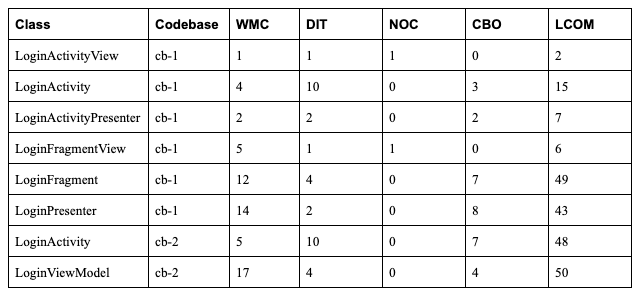
\includegraphics[scale=0.5]{figures/login-metric-table.png}
    \caption{CodeMR Metric Values for Login Feature} 
    \label{fig:login-metric-table}
\end{table}

In order to examine the results better, groupings can be made between these classes, and the metric values of these groups can be compared. This grouping can be made based on the responsibilities of the classes. The responsibilities to be taken as a basis while determining groups are the view and view presentation. More detailed information on these responsibilities was shared in previous sections. These classes and their interfaces can be grouped for each codebase as follows. For CB-1, LoginActivityView, LoginActivity, LoginFragmentView and LoginFragment are only responsible for the view responsibility.  LoginActivityPresenter and LoginFragmentPresenter are the classes responsible for how and when the data is presented. For CB-2, LoginActivity is responsible for the view responsibility, and LoginViewModel is responsible for how and when data is presented. This grouping will be useful for comparing the metric values shared in Table \ref{fig:login-metric-table}. Table \ref{fig:login-metric-table-2} presents the metric values for each group of both codebases that are obtained from the analysis.

\begin{table}[htb]
    \centering
    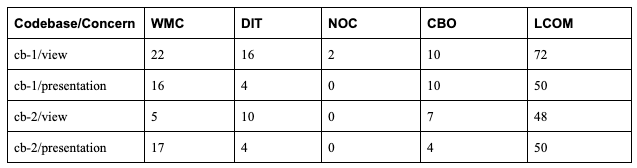
\includegraphics[scale=0.5]{figures/login-metric-table-2.png}
    \caption{CodeMR Metric Values for Login Feature}
    \label{fig:login-metric-table-2}
\end{table}

Results showed that the CB-1 codebase uses 6 entities for the selected layers of the login feature, while CB-2 uses only 2. From this point of view, the CB-2 has better organization and understandability. Moreover, when the values of WMC, DIT and NOC metrics used in complexity measurement are compared, it is seen that the complexity level of CB-2 for the view responsibility is lower. On the other hand, when the results of the complexity metric values of presentation related responsibilities are examined, it is observed that there is not much difference between the two code bases. These results should be considered normal given the complexity of functionality of the classes involved in this responsibility. When the CBO metric related to measuring the coupling level is examined, it is seen that the CB-2 codebase gives better results. Since the SOLID and DI principles are used much more effectively in the CB-2 codebase, these results are expected. Also, CB-1 uses the MVP design pattern. The coupling of the CB-1 is increasing due to the bi-directional dependency between view and presentation layers in the MVP design pattern. However, this situation is not the case for CB-2, which uses the MVVM design pattern. In the MVVM design pattern, only the view layer has a dependency on the presentation layer. When the results of the LCOM metric related to cohesion are examined, it is seen that the results are similar to the results of the complexity metrics. While the results of CB-2 are much better than CB-1 for the responsibility of view, there is not much difference between the results for the responsibility of presentation. There is only one view model per view principle in the MVVM design pattern. Therefore, one view model might have different responsibilities, especially those that belong to the complex views. The same is true for the MVP design pattern as well. There can be only one presenter for each view. Naturally, CB-1, which uses the MVP design pattern, seems to have low cohesion values for presentation responsibility. 